% Created 2014-12-02 Tue 16:56
\documentclass[presentation]{beamer}
\usepackage[utf8]{inputenc}
\usepackage[T1]{fontenc}
\usepackage{fixltx2e}
\usepackage{graphicx}
\usepackage{longtable}
\usepackage{float}
\usepackage{wrapfig}
\usepackage{rotating}
\usepackage[normalem]{ulem}
\usepackage{amsmath}
\usepackage{textcomp}
\usepackage{marvosym}
\usepackage{wasysym}
\usepackage{amssymb}
\usepackage{hyperref}
\tolerance=1000
\usetheme{default}
\author{Üstün Özgür}
\date{2 Aralık 2014}
\title{Emacs'e Giriş}
\hypersetup{
  pdfkeywords={},
  pdfsubject={},
  pdfcreator={Emacs 24.4.1 (Org mode 8.2.10)}}
\begin{document}

\maketitle


\begin{frame}[label=sec-1]{Emacs}
\begin{quote}
Emacs is the extensible, customizable, self-documenting real-time display
editor.
\end{quote}

\begin{block}{Extensible}
\end{block}
\begin{block}{Customizable}
\end{block}
\begin{block}{Self-documenting}
\end{block}
\end{frame}

\begin{frame}[label=sec-2]{Tarihçe}
\begin{itemize}
\item 1970'lerde Richard Stallman tarafından yazıldı
\item James Gosling tarafından ilk Unix uyarlaması
\item 1980'lerde GNU projesi ve GNU Emacs
\item Isletim sistemi ile iletişimi sağlayan küçük C çekirdeği
\item Çekirdeğin üzerinde çalışan Emacs Lisp motoru
\end{itemize}

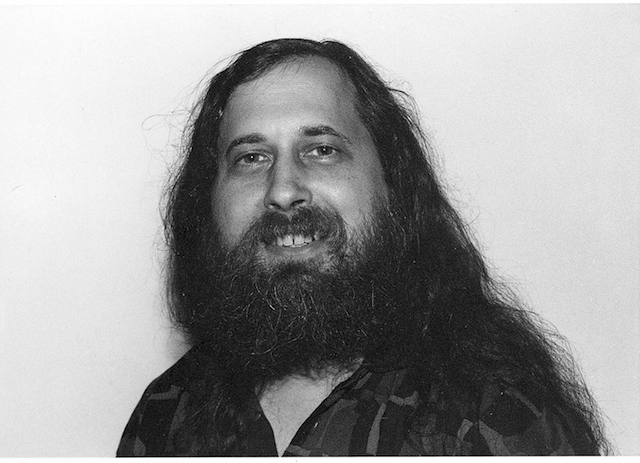
\includegraphics[width=.9\linewidth]{./images/stall.jpg}
\end{frame}

\begin{frame}[label=sec-3]{Emacs bir metin editörü değildir}
\begin{itemize}
\item Emacs bir programlama ortamıdır
\end{itemize}
\begin{quote}
GNU Emacs is sometimes called an "extensible editor", but it does
much more than provide editing capabilities.  It is better to refer to
Emacs as an "extensible computing environment".  However, that phrase
is quite a mouthful.  It is easier to refer to Emacs simply as an
editor.
\end{quote}

\begin{itemize}
\item Komutlar (command), fonksiyon ve değişkenler
\item M-x : Emacs'ın en önemli komutu
\end{itemize}
\end{frame}

\begin{frame}[label=sec-4]{Giriş: Bir metin editörünün temel görevleri}
\begin{itemize}
\item Dosya ve pencere yönetimi
\item Dosyanın içeriğinini değiştirme
\item Dosyanın içerisinde hareket etme
\item Dosyalar arasında hareket etme
\item Dosya üzerinde bir işlem yapma (compile, spell-check)
\end{itemize}
\end{frame}

\begin{frame}[label=sec-5]{User Interface}
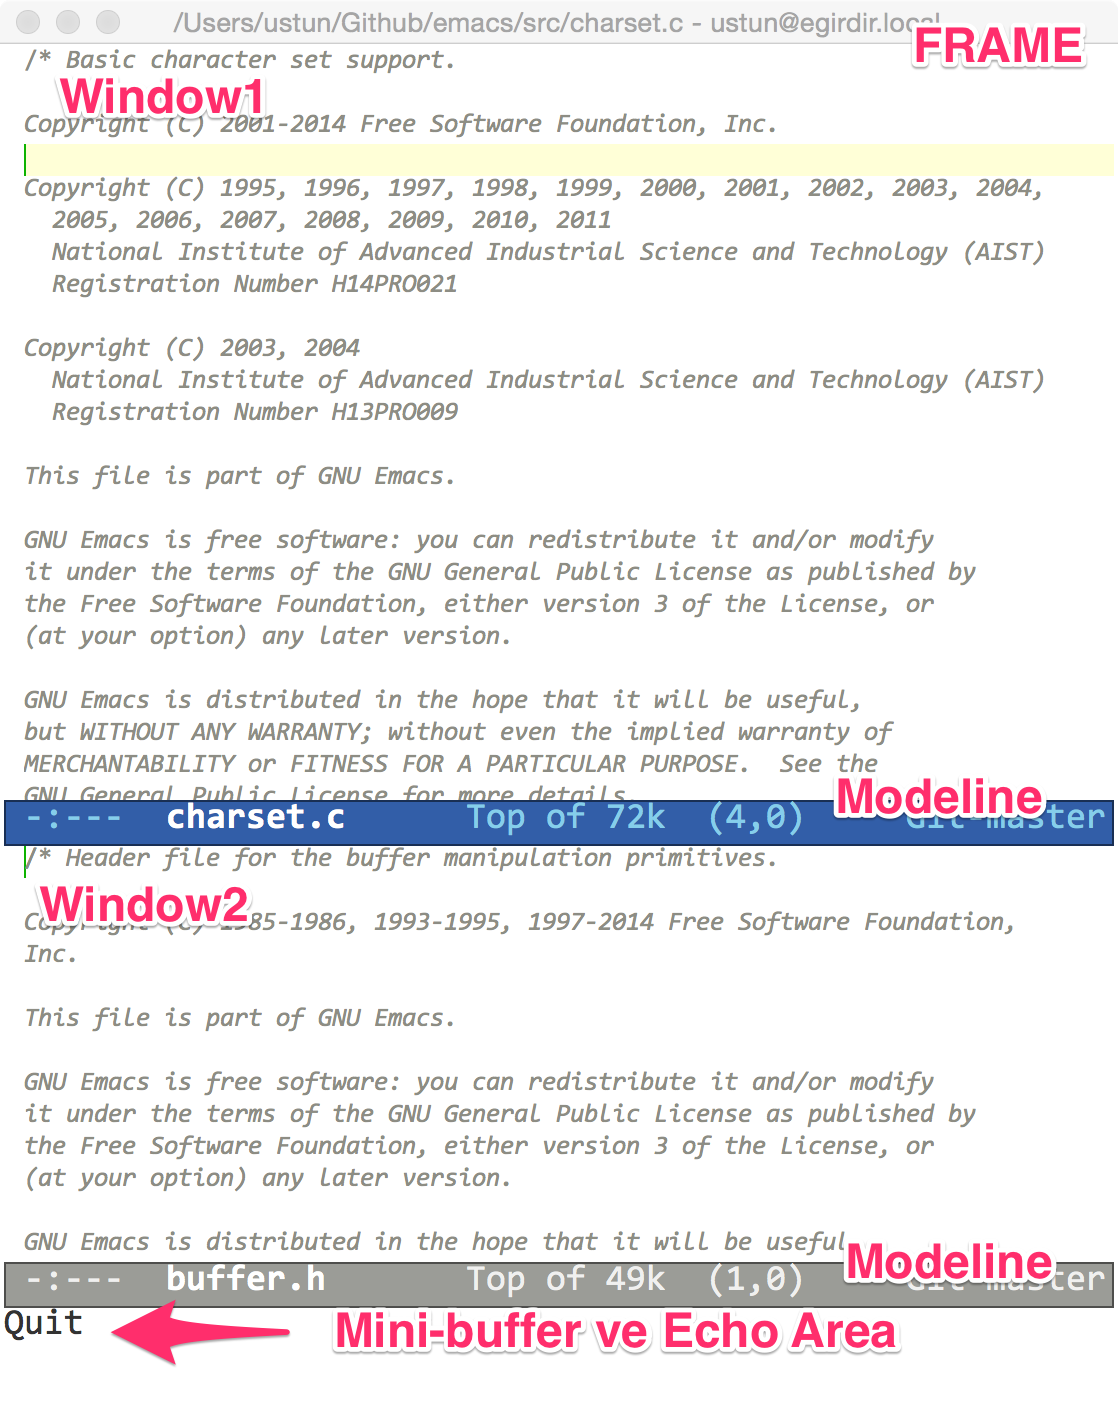
\includegraphics[width=5cm]{./images/emacs.png}
\end{frame}

\begin{frame}[label=sec-6]{Temel Kavramlar}
\begin{itemize}
\item Frame (pencere)
\item window (bölme)
\item buffer (metin -- dosya olabilir ya da olmayabilir
\item mini-buffer ve echo area (en alttaki alan)
\end{itemize}
\end{frame}

\begin{frame}[label=sec-7]{Demo}
\begin{itemize}
\item find-file
\item split-window-vertically
\item split-window-horizontally
\item delete-other-windows
\item dired
\item kill-buffer
\item switch-to-buffer
\item insert
\item beginning-of-line
\item end-of-line
\item previous-line
\item forward-line
\item upcase-region
\item undo
\end{itemize}
\end{frame}

\begin{frame}[label=sec-8]{Temel Komutlar}
\begin{itemize}
\item Dosya açma/kapama
\begin{itemize}
\item C-x C-f : Find file
\item C-x C-b : Açık dosyalar ve bufferlar
\item C-x C-s : Kaydetme
\item C-x C-k : Kapatma
\end{itemize}

\item Pencere yönetimi
\begin{itemize}
\item C-x 2 : Yatay olarak ikiye bölme
\item C-x 3:  Dikey olarak ikiye bölme
\item C-x 1:  Diğer bölmeleri kapatma
\end{itemize}

\item Hareket tuslari:
\begin{itemize}
\item C-a/e/f/b: Satir basi/sonu/bir harf ileri/bir harf geri
\item M-a/e/f/b: Para basi/sonu/bir kelime ileri/bir kelime geri
\end{itemize}
\end{itemize}
\end{frame}

\begin{frame}[label=sec-9]{Nasıl Öğrenebilirsiniz?}
\begin{itemize}
\item Self-documenting
\item C-h t : Emacs tutorial
\item C-h r : Emacs manual
\item C-h i : Emacs Lisp Info
\item Emacs Prelude
\end{itemize}
\end{frame}

\begin{frame}[label=sec-10]{Özelleştirme}
\begin{itemize}
\item init dosyasi
\item M-x customize
\item M-x customize-variable
\item M-x define-variable
\item M-x define-function
\item M-x find-function
\item M-x find-library
\end{itemize}
\end{frame}

\begin{frame}[label=sec-11]{Sorular}
\begin{itemize}
\item @ustunozgur
\item ustun@ustunozgur.com
\item github.com/ustun/emacs-sunum
\end{itemize}
\end{frame}
% Emacs 24.4.1 (Org mode 8.2.10)
\end{document}
